\counterwithin{figure}{section}
\chapter{Risultati sperimentali e analisi}

\section{Parametri utilizzati}
Sono state effettuate simulazioni prendendo in esame 4 delle 10 scuderie disponibili. In tre di queste l’obiettivo è quello di individuare il miglior asset di investimento, nella quarta invece è quello di analizzare quanto l’introduzione di un nuovo pilota possa incidere sul risultato finale. 
Per le prime tre simulazioni, per ognuno dei team, sono stati utilizzati 27 diversi asset (Figura~\ref{fig:asset}) di investimenti per la comparazione. 
 
\begin{figure}[H]
    \centering
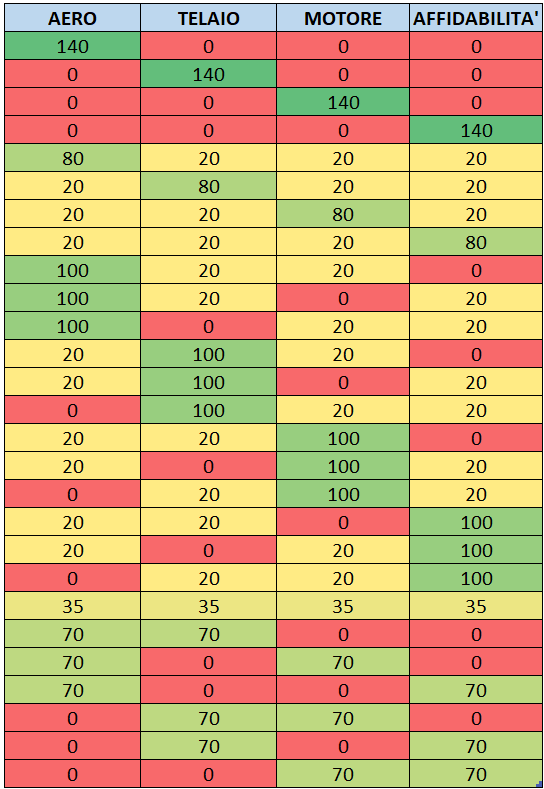
\includegraphics[width=0.7\textwidth, height=9.6cm]{Figures/asset.png} 
    \caption{Tabella degli asset scelti per svolgere le simulazioni}
    \label{fig:asset}
\end{figure}

La tabella in Figura~\ref{fig:asset} utilizza una codifica che utilizza un gradiente di colori per rappresentare i valori numerici e facilitare l'interpretazione visiva dei dati, permettendo di identificare rapidamente i valori più significativi. La legenda dei colori è la seguente:
\begin{itemize}
    \item Verde : Valori alti;
    \item Giallo : Valori bassi;
    \item Rosso : Valori nulli.
\end{itemize}
Questa codifica facilita l'interpretazione visiva dei dati, permettendo di identificare rapidamente i valori più significativi.

\newpage

\section{Variabilità dei dati}
Inoltre, al fine di ridurre l'influenza della variabilità delle singole simulazioni, ogni asset viene valutato sulla base della media di due simulazioni indipendenti.

È importante sottolineare che le simulazioni possono mostrare risultati significativamente diversi anche quando vengono eseguite con gli stessi parametri in input, a causa delle molte variabili casuali coinvolte nel processo.

A titolo esemplificativo, sono state condotte 20 simulazioni utilizzando gli stessi parametri di input per la Scuderia Ferrari.
 
\begin{figure}[h]
    \centering
    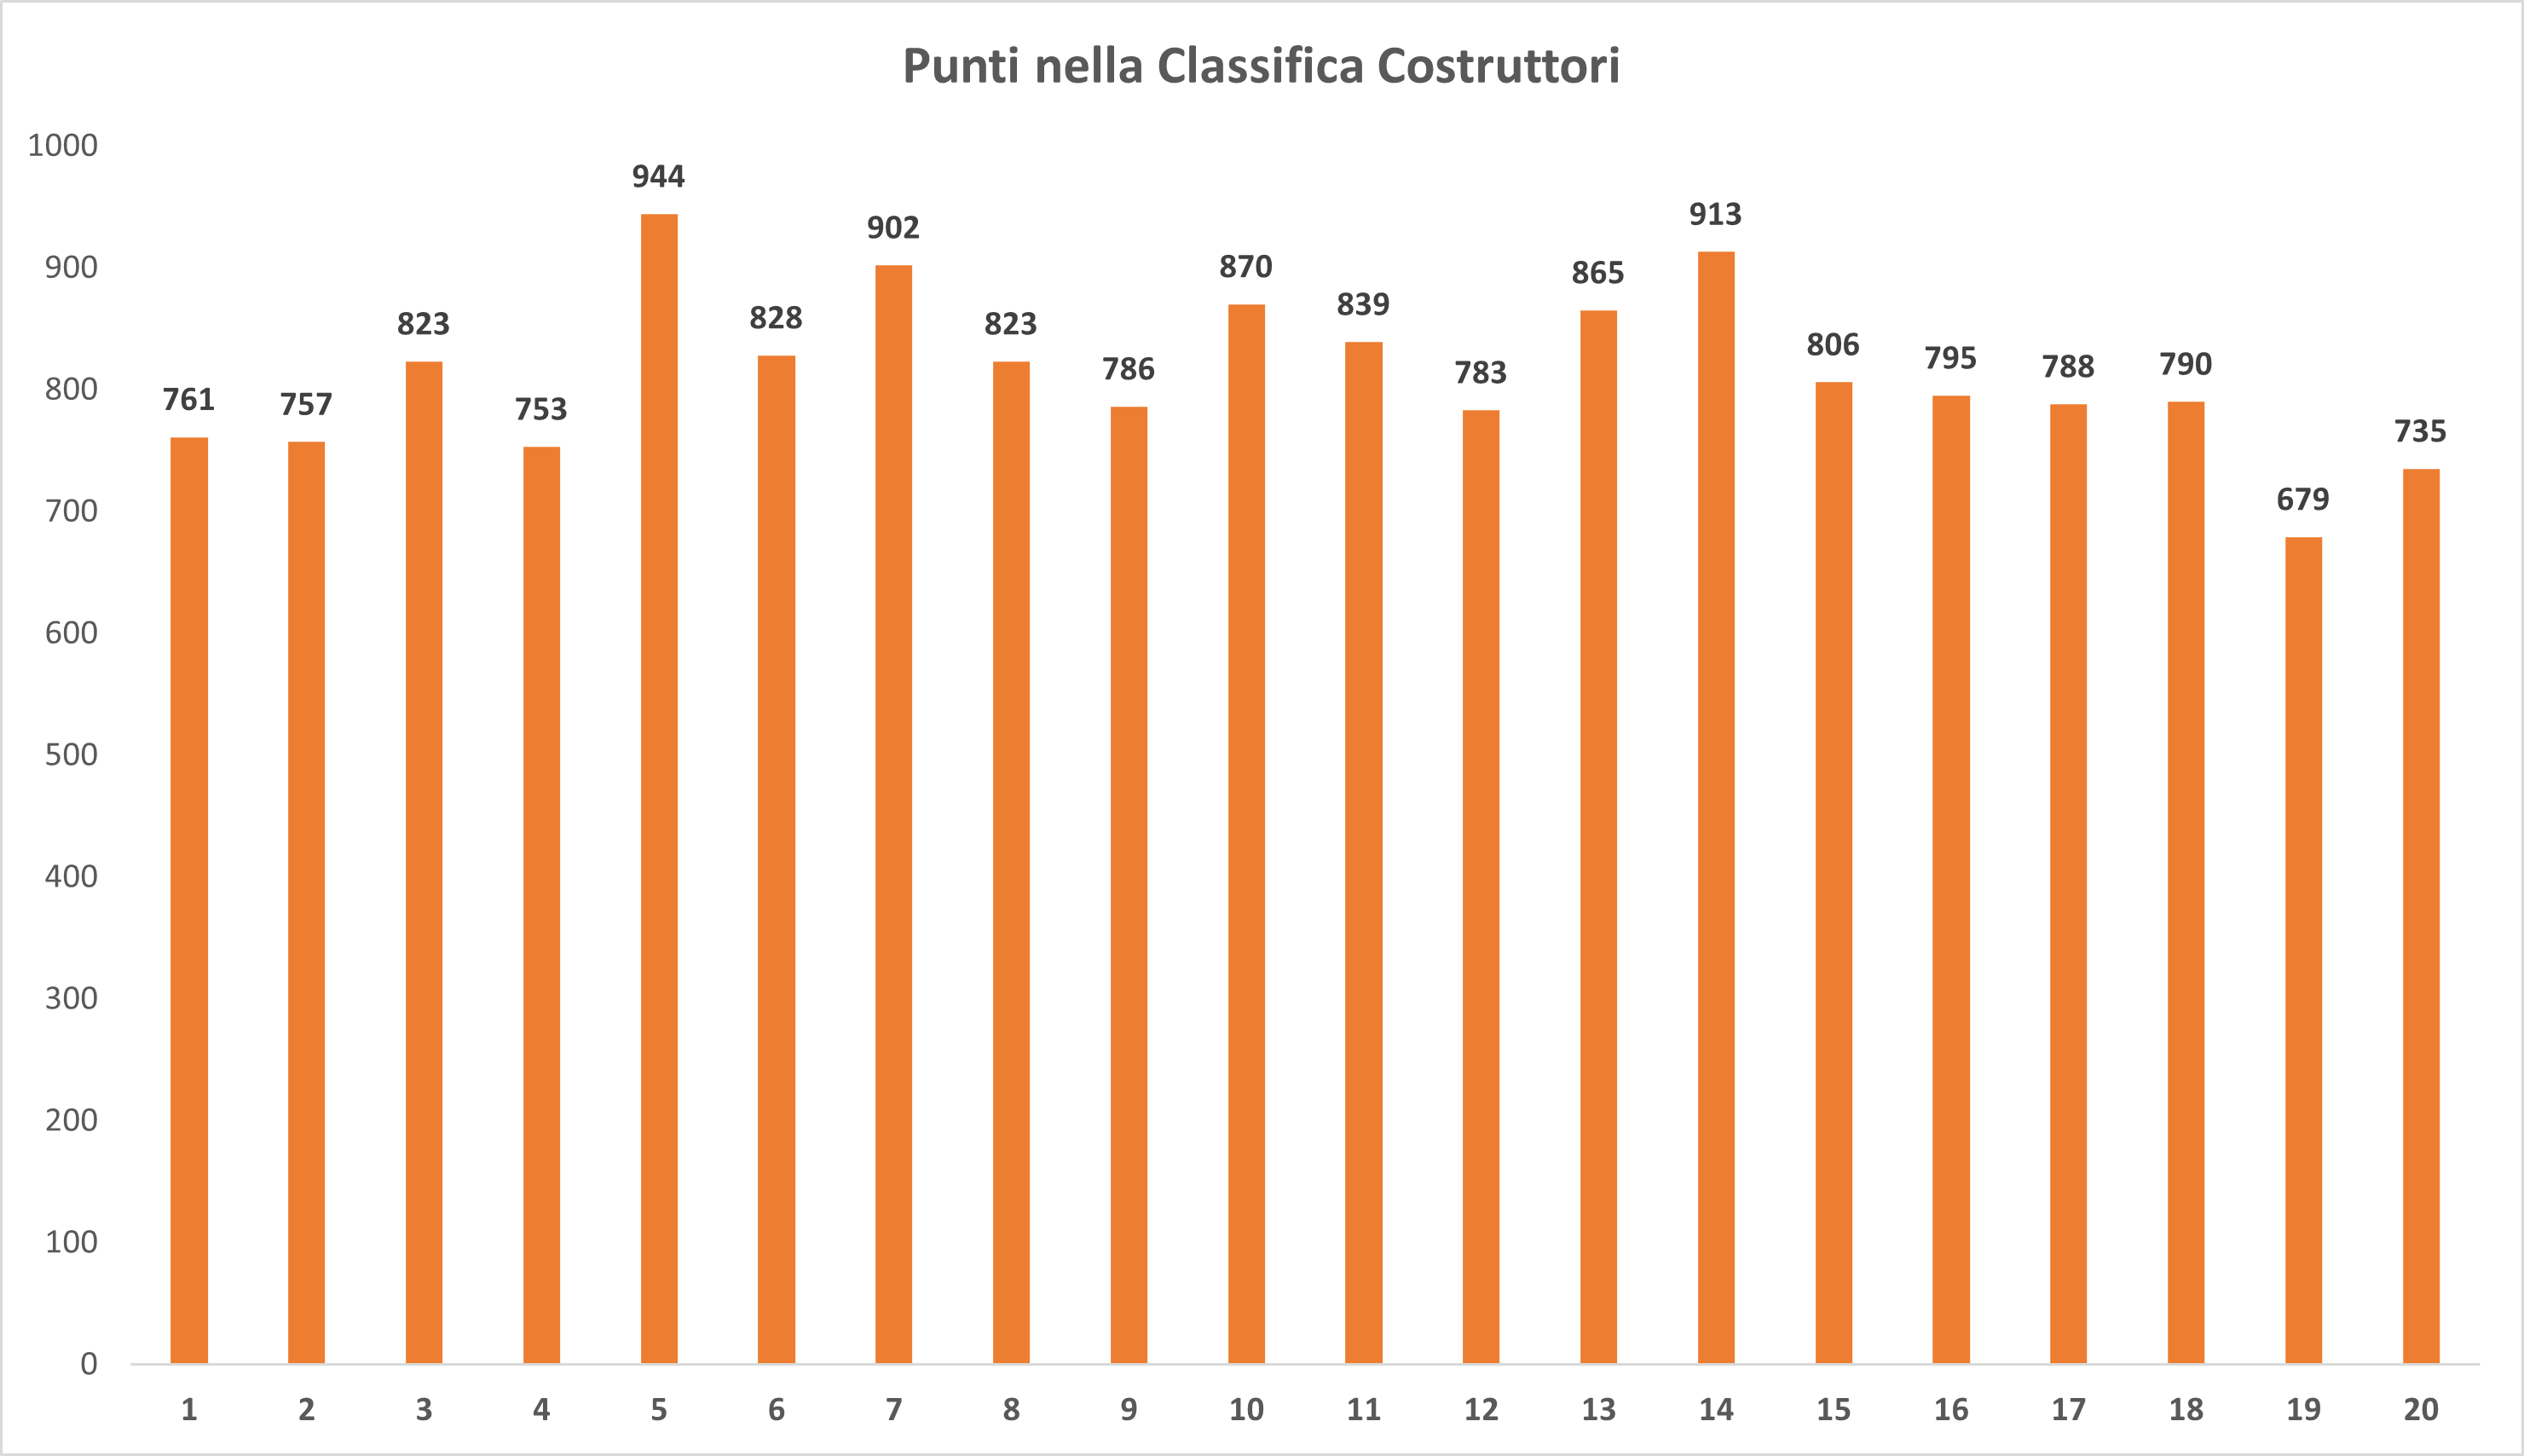
\includegraphics[width=\textwidth]{Figures/fvar.png}
    \caption{Grafico a barre dei risultati della simulazione con Scuderia Ferrari utilizzando lo stesso asset di investimenti}
    \label{fig:ferrari}
\end{figure}

I risultati numerici delle 20 simulazioni costituiscono una popolazione di campioni. Tra questi, il valore massimo ottenuto è stato di 944 punti, mentre il valore minimo è stato di 679 punti, con una differenza di 265 punti tra i due estremi.

La media dei risultati ottenuti è stata di 812 punti, con una deviazione standard\footnote{dettagli aggiuntivi nell'Appendice~\ref{appendice:ds}} di 64.38 punti e un coefficiente di variabilità\footnote{dettagli aggiuntivi nell'Appendice~\ref{appendice:cv}} del 8%.

Questi dati evidenziano una variabilità significativa nei risultati delle simulazioni, anche quando vengono utilizzati gli stessi parametri di input.



\newpage
\section{Simulazione Ferrari}

\begin{figure}[h]
    \centering
    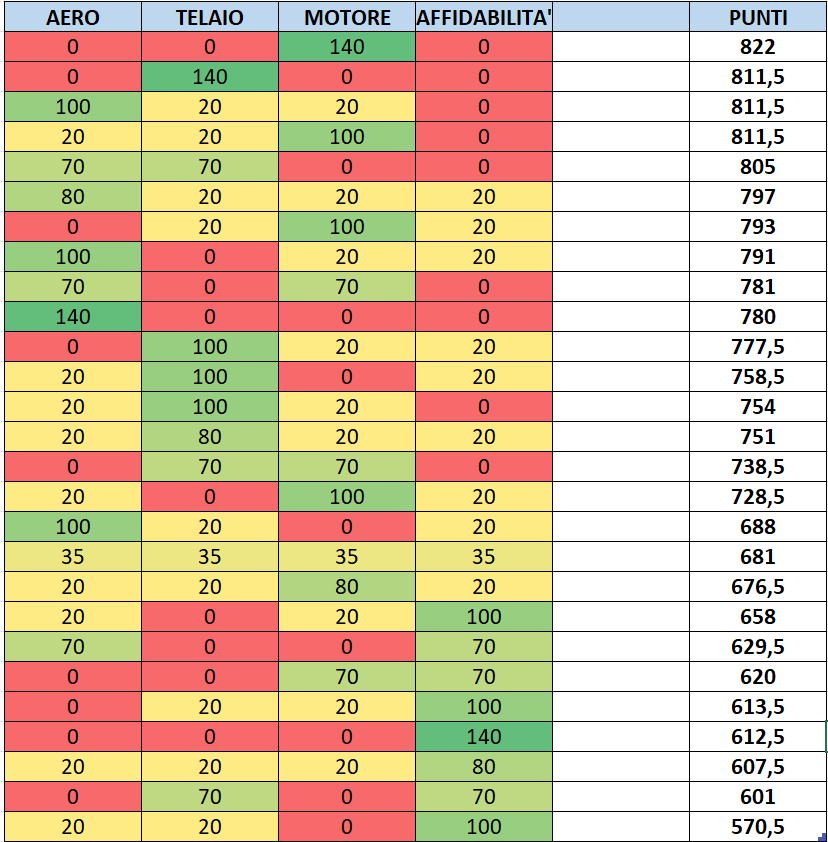
\includegraphics[width=\textwidth, height=11cm]{Figures/ferrari1.png} 
    \caption{Tabella che riporta i risultati della simulazione con la Scuderia Ferrari usando i 27 diversi asset di investimento}
    \label{fig:ferrari_assets}
\end{figure}

Dai risultati riportati nella Figura~\ref{fig:ferrari_assets}, si osserva che il massimo punteggio raggiungibile per il team Ferrari si aggira attorno agli 800 punti. Guardando le migliori cinque simulazioni, emerge chiaramente che un investimento nel settore dell’Affidabilità non è vantaggioso per il team. La tabella mostra una distribuzione prevalentemente negativa (cellule verdi in basso), indicando risultati inferiori.

Escluso il settore dell’Affidabilità, gli altri tre sembrano poter incidere in maniera simile sul risultato finale, ma tramite il calcolo del IPCI\footnote{dettagli aggiuntivi nell'Appendice~\ref{appendice:ipci}}(Figura~\ref{fig:ipci}) si intuisce come l’ambito Telaio sia leggermente meno significativo degli altri due. 


\begin{figure}[h]
    \centering
    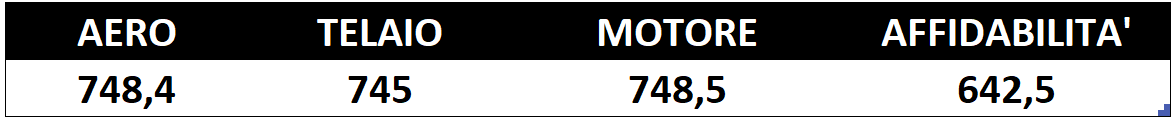
\includegraphics[width=\textwidth]{Figures/ferrari2.png} % sostituire con il nome del file immagine
    \caption{Tabella che riporta il valore IPCI dei vari reparti in cui è possibile investire con la scuderia Ferrari}
    \label{fig:ipci}
\end{figure}

In conclusione, le migliori strategie per il team Ferrari sembrano essere due: investire la totalità del budget nel settore motoristico o ripartire le risorse tra le tre aree Telaio, Motore e Aerodinamica.

\newpage

\section{Simulazione Alpine}

\begin{figure}[h]
    \centering
    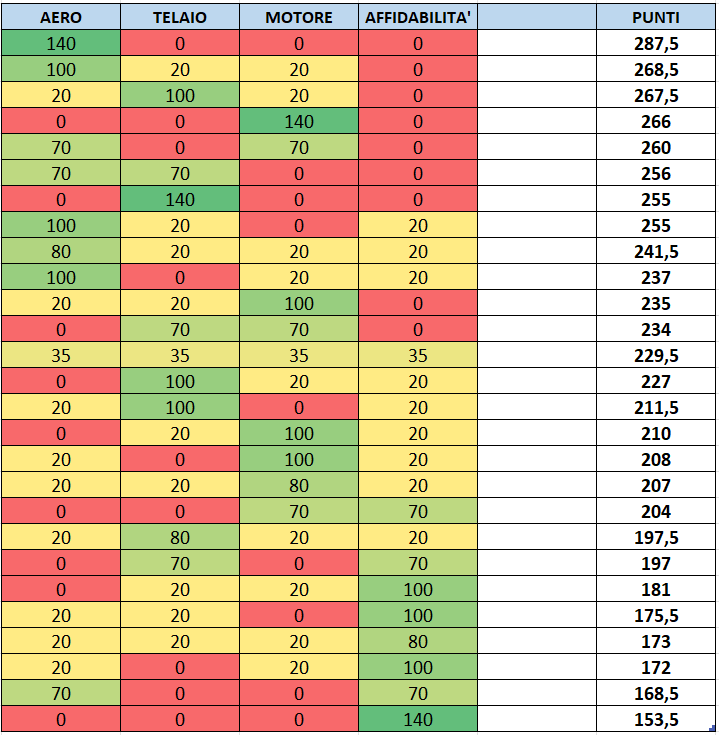
\includegraphics[width=\textwidth, height = 11cm]{Figures/alpine1.png}
    \caption{Tabella dei risultati della simulazione con la Scuderia Alpine usando i 27 diversi asset di investimento}
    \label{fig:figura9_5}
\end{figure}

\begin{figure}[h]
    \centering
    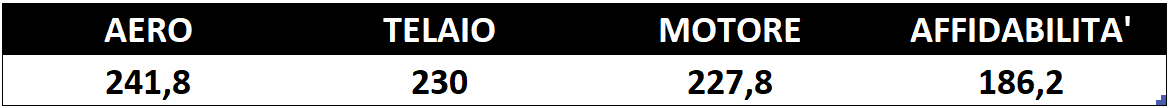
\includegraphics[width=\textwidth]{Figures/alpine2.png}
    \caption{Tabella del valore IPCI dei vari reparti in cui è possibile investire con la Scuderia Alpine}
    \label{fig:figura9_6}
\end{figure}

Dai risultati riportati nella Figura~\ref{fig:figura9_5} è facile notare quanto un investimento nel settore dell’affidabilità sia poco producente in termini di punti nella classifica finale. Infatti, le migliori sette simulazioni riportate indicano un investimento nullo in tale settore.

Per quanto riguarda gli altri tre settori, tramite una semplice analisi visiva della Figura~\ref{fig:figura9_5} si potrebbe intuire che ce ne sia uno più vantaggioso di altri in cui investire: quello Aerodinamico. Ciò è confermato anche dal confronto dei valori di IPCI\footnote{dettagli aggiuntivi nell'Appendice~\ref{appendice:ipci}} (Figura~\ref{fig:figura9_6}): il settore dell’Aerodinamica ha più di 11 punti rispetto a Telaio e Motore, che risultano essere comparabili in termini di rendimento.

Si evince quindi che la miglior strategia di investimento per il team Alpine sia quella di investire la totalità del budget o quasi nel settore dell’aerodinamica. Questa strategia permetterebbe al team di raggiungere un punteggio che si aggira intorno ai 290 punti.

\newpage

\section{Simulazione Haas}

\begin{figure}[h]
    \centering
    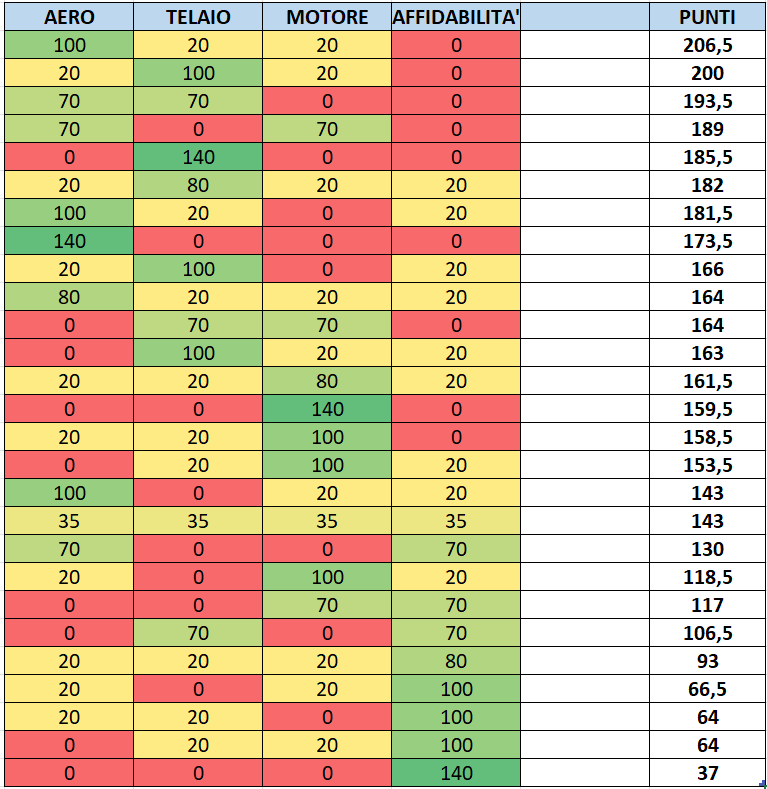
\includegraphics[width=\textwidth, height=11cm]{Figures/haas1.png}
    \caption{Tabella dei risultati della simulazione con la Scuderia Haas usando i 27 diversi asset di investimento}
    \label{fig:figura9_7}
\end{figure}

Per quanto riguarda la scuderia Haas, dall’analisi della tabella mostrata in Figura~\ref{fig:figura9_7}, si riconferma il fatto che un investimento nell’affidabilità non è fruttuoso. Del resto, dal confronto tra le varie aree si può notare come la distribuzione dei colori nella tabella indichi che un investimento nel settore Motore sia meno vantaggioso che nei settori Aerodinamica e Affidabilità. Infatti, confrontando i valori di IPCI\footnote{dettagli aggiuntivi nell'Appendice~\ref{appendice:ipci}} si nota come Aerodinamica e Telaio abbiano un punteggio molto simile e il settore del Motore sia staccato di circa 16 punti. Fanalino di coda l’Affidabilità, lontana dai punteggi degli altri settori.

\begin{figure}[h]
    \centering
    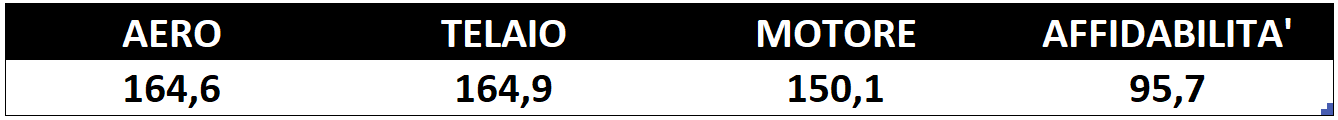
\includegraphics[width=\textwidth]{Figures/haas2.png}
    \caption{Tabella del valore IPCI dei vari reparti in cui è possibile investire con la scuderia Haas}
    \label{fig:figura9_8}
\end{figure}

Dai dati ricavati dalle varie simulazioni si giunge alla conclusione che la miglior strategia d’investimento per il team Haas è quella di concentrare l’intero budget tra i settori di Aerodinamica e Telaio.

\newpage

\section{Analisi Aston Martin}

In questa simulazione non sono stati apportati investimenti tecnici al team ma è stato sostituito un pilota del team, Lance Stroll (dodicesimo pilota per overall), con Max Verstappen (primo pilota per overall). Sono state effettuate 15 simulazioni per coppia di piloti:
\begin{itemize}
    \item Coppia standard: Fernando Alonso – Lance Stroll;
    \item Coppia sperimentale: Fernando Alonso – Max Verstappen.
\end{itemize}




\begin{figure}[h]
    \centering
    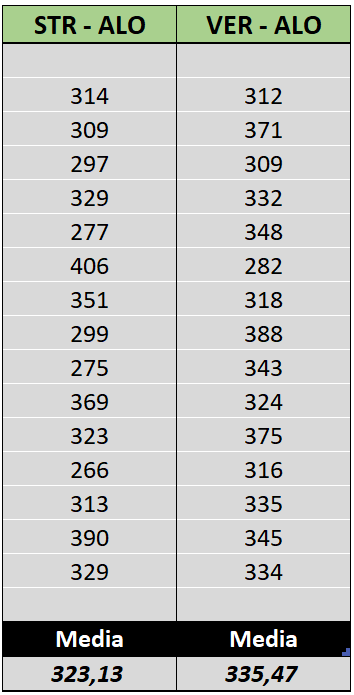
\includegraphics[width=0.5\textwidth, height = 9cm]{Figures/piloti.png}
    \caption{Tabella che riporta il confronto dei risultati delle simulazioni della Scuderia Aston Martin con una diversa coppia di piloti}
    \label{fig:figura9_9}
\end{figure}

Nonostante una netta differenza tra overall tra Max Verstappen (90,75) e Lance Stroll (83,05), i risultati finali non discostano di molto. La media dei punteggi ottenuti dimostra che a fronte di un cambio pilota che ha apportato un incremento di 8.7 nell’overall del pilota, il punteggio finale nella classifica costruttori è aumentato solo di 12,34 punti in media. Quindi la sostituzione del pilota Lance Stroll con il pilota più abile Max Verstappen non risulta essere particolarmente significativa per la classifica finale della scuderia Aston Martin.

\newpage

\section{Analisi finale}

In conclusione, un’osservazione ricorrente nelle prime tre simulazioni è che un investimento nel settore legato all’Affidabilità non ha un buon ritorno in termini di punti nella classifica costruttori, soprattutto per i team nella parte bassa della classifica. I dati evidenziano che è più vantaggioso concentrarsi sullo sviluppo dei settori che migliorano le prestazioni andando a ridurre i tempi sul giro, piuttosto che sviluppare un settore che mitiga i rischi legati ai guasti tecnici e che costringerebbero la vettura al ritiro. Relativamente agli altri settori, la strategia varia significativamente da scuderia a scuderia, poiché ciascuna ha un bilanciamento unico tra i reparti tecnici. Sebbene le tre simulazioni abbiano mostrato che l’Aerodinamica tende a garantire un buon tasso di rendimento, è importante notare che questa osservazione potrebbe non essere universalmente valida per tutte le dieci scuderie. Le simulazioni effettuate utilizzando un ampio numero di asset hanno permesso di individuare strategie particolarmente fruttuose per i team presi in considerazione. Tuttavia, per aumentare l'efficacia della ricerca, sarebbe necessario esplorare un numero molto maggiore di combinazioni di investimento e condurre simulazioni più approfondite per ciascuna di esse, al fine di ridurre la variabilità degli output e ottenere risultati più solidi e generalizzabili. Per quanto riguarda l’opportunità di poter cambiare i piloti della propria squadra, si è osservato che nel caso di Aston Martin, nonostante una sostituzione importate, non si è registrato un gran incremento di punti nella classifica finale. Al fine di valutare al meglio quanto un cambio pilota possa influire sul punteggio finale di una scuderia, è necessario effettuare simulazioni con diverse scuderie, soprattutto quelle posizionate nella parte bassa della classifica che potrebbero avere valori tecnici simili tra loro.






